\documentclass[../Head/Main.tex]{subfiles}
\begin{document}
\subsection{HLS Histogram}
\label{subsec:test_HLS_hist}
The purpose of this test was to find the hue value of the blue marbles, in order to convert the image to a black and white. 

\subsubsection{Description of test}



\subsubsection{Test parameters}
\begin{minipage}[c]{0.35\textwidth}
	\begin{tabular}{l r}
	- World used                   & 5-room world\\
	- Initial room                 & room 3\\	
	- Probabilities based on       & 50 tests\\	
	- Number of tests              & 100\\
	- Scaling factor distance      & 1.2\\
	- Scaling factor reward        & 20\\
	- Randomness factor $\epsilon$ & 0.05\\
	- Discount factor $\gamma$     & 0.9\\
	\end{tabular}
\end{minipage}	

\subsubsection{Data}


\begin{figure}[H]
	\centering
	\begin{subfigure}[b]{0.48\textwidth}
		\centering
		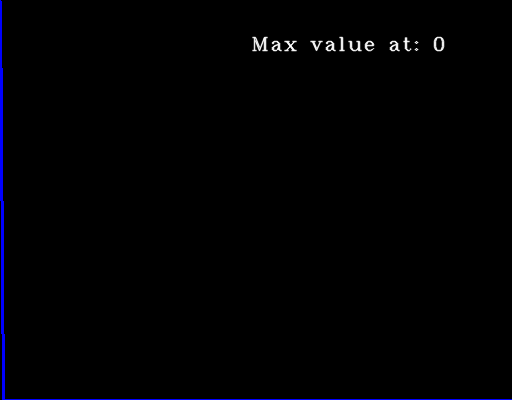
\includegraphics[width=\textwidth]{CV/camera_hls_histogram_1}
		\caption{caption}
	\end{subfigure}
	\hfill
	\begin{subfigure}[b]{0.5\textwidth}
		\centering
		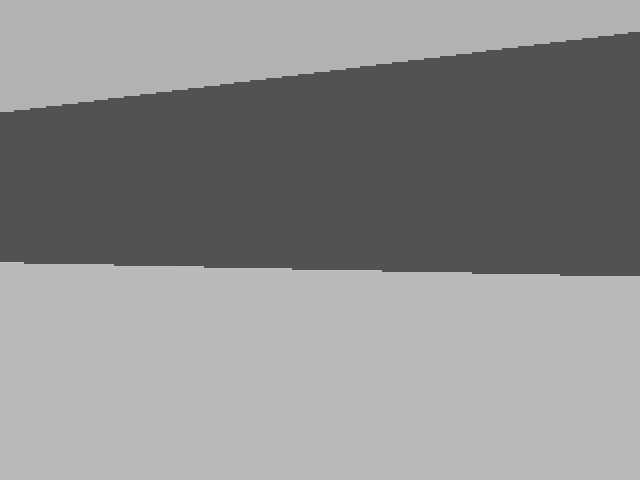
\includegraphics[width=\textwidth]{CV/camera_test_image_1}
		\caption{caption}
	\end{subfigure}
	\caption{caption}
\end{figure}

\begin{figure}[H]
	\centering
	\begin{subfigure}[b]{0.48\textwidth}
		\centering
		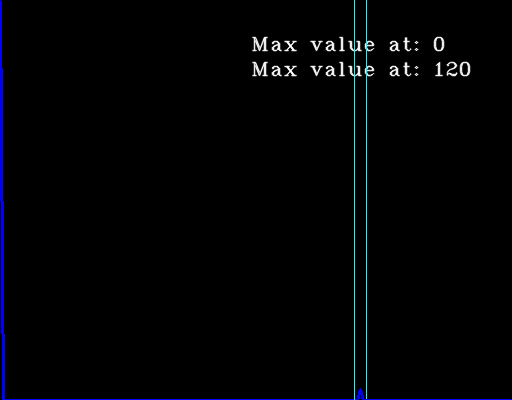
\includegraphics[width=\textwidth]{CV/camera_hls_histogram_2}
		\caption{caption}
	\end{subfigure}
	\hfill
	\begin{subfigure}[b]{0.5\textwidth}
		\centering
		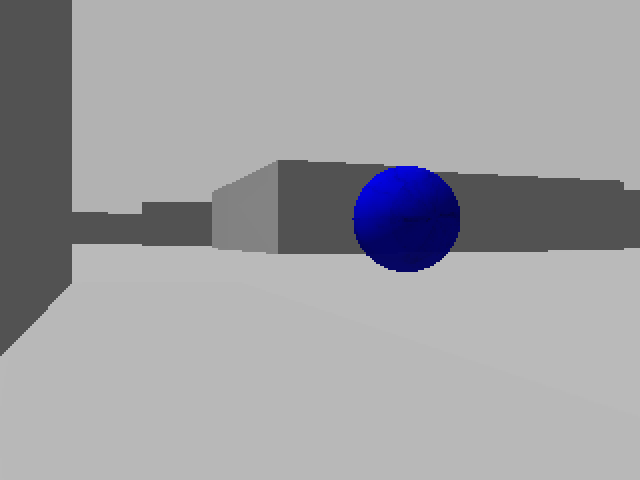
\includegraphics[width=\textwidth]{CV/camera_test_image_2}
		\caption{caption}
	\end{subfigure}
	\caption{caption}
\end{figure}

\begin{figure}[H]
	\centering
	\begin{subfigure}[b]{0.48\textwidth}
		\centering
		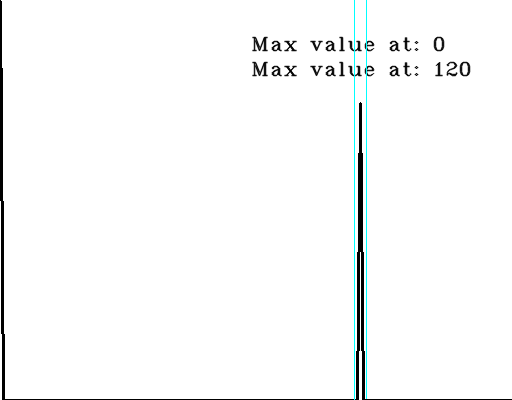
\includegraphics[width=\textwidth]{CV/camera_hls_histogram_5}
		\caption{caption}
	\end{subfigure}
	\hfill
	\begin{subfigure}[b]{0.5\textwidth}
		\centering
		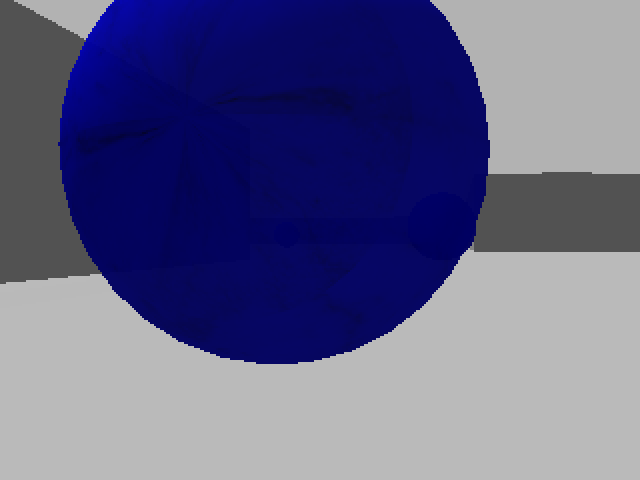
\includegraphics[width=\textwidth]{CV/camera_test_image_5}
		\caption{caption}
	\end{subfigure}
	\caption{caption}
\end{figure}

\subsubsection{Conclusion}
The value of 120 was chosen as the threshold 

\end{document}